\documentclass[journal]{IEEEtran}

\usepackage{cite}
\usepackage{amsmath,amssymb}
\usepackage{graphicx}
\usepackage{array}
\usepackage{tikz}
\usetikzlibrary{arrows.meta,positioning,shapes.geometric,fit,calc}
\usepackage{url}
\usepackage[hidelinks]{hyperref}

\graphicspath{{figures/}}
\hyphenation{re-luc-tance pe-de-lec}

\begin{document}

\title{Analysis and Design Considerations for a Switched Reluctance Motor-Based Drive System for an Electric Bike}

% TODO: replace with the actual author list, affiliations and funding note.
\author{First~A.~Author,~\IEEEmembership{Member,~IEEE,}
        Second~B.~Author,
        and~Third~C.~Author%
\thanks{Manuscript received XXXX; revised XXXX.}%
\thanks{The authors are with the Department of Electrical and Electronics Engineering, XXXX, India (e-mail: author@institution.edu).}%
\thanks{The simulation toolchain used in this work is available as open source in the accompanying repository.}}

\markboth{IEEE Transactions on Transportation Electrification,~Vol.~XX, No.~X, Month~2026}%
{Author \MakeLowercase{\textit{et al.}}: SRM-Based Drive System for an Electric Bike}

\maketitle

\begin{abstract}
Switched reluctance motors (SRMs) are magnet-free, mechanically robust and
cost-effective. They also produce no drag torque when unpowered, which makes
them attractive for light electric vehicles. This paper presents a systematic
analysis and design of an SRM drive for a \mbox{250-W}, 25-km/h pedelec supplied
from a 36-V battery. The vehicle mission is translated into motor
torque--speed requirements. We show that the turns must be chosen at a
\emph{corner speed} rather than at the assist cut-off speed, and we derive the
relation $P_c = k_c V_{dc} I_{pk}$. This relation implies that the peak phase
current depends only weakly on machine size. A 12/8 three-phase machine
is sized from the output equation, the feasible pole-arc region and the
volt-second balance. It is evaluated with a saturable flux-linkage model coupled
to a time-domain model of an asymmetric half-bridge converter, and the
turn-on angle, turn-off angle and current reference are optimized at every
operating point. The resulting $\varnothing$135-mm, 3.4-kg (active) design,
coupled to an 8:1 planetary gear, delivers the 5.9-N$\cdot$m launch torque at
31~A. It reaches 75.8\% motor efficiency and 72.8\% battery-to-shaft efficiency
at the rated point, and consumes 5.05~Wh/km on a hilly urban route. A trade
study over gear ratio and electric loading quantifies the
efficiency--mass--gearing compromise. Converter ratings, the DC-link
capacitor, thermal behavior, torque ripple and position sensing are also discussed.
\end{abstract}

\begin{IEEEkeywords}
Asymmetric half-bridge converter, electric bicycle, light electric vehicle,
machine design, pedelec, switched reluctance motor (SRM), torque ripple.
\end{IEEEkeywords}

\section{Introduction}
\IEEEPARstart{E}{lectric} bicycles are the most widely sold electric vehicles
worldwide. Their drives are almost exclusively brushless permanent-magnet (PM)
hub or mid-drive motors. PM machines offer high torque density and
efficiency, but they rely on rare-earth magnets. Those magnets carry supply-chain and price
risk, limit operating temperature and add drag torque when unpowered (cogging
and eddy-current losses). This last point matters for a pedelec,
which by regulation must be pedaled and is ridden unassisted above
25~km/h~\cite{en15194}.

The switched reluctance motor (SRM) addresses these concerns. Its rotor is a
stack of laminations, its stator carries concentrated coils, and its phases
are electrically and magnetically independent. This gives inherent fault
tolerance and zero torque when the windings are not excited~\cite{miller1993,krishnan2001}.
SRMs have been studied extensively for electric and hybrid
vehicles~\cite{rahman2000,xue2010,jiang2017,bilgin2019}. Their known drawbacks
are torque ripple, acoustic noise and lower efficiency at small power
ratings~\cite{husain2002,vujicic2012}. Classical design procedures~\cite{krishnan1988,radun1995,vijayakumar2008}
and pole-number studies~\cite{bilgin2012} exist. However, most target
kilowatt-to-hundred-kilowatt machines with relatively high DC-link voltages.
The \mbox{250-W}, 36-V pedelec regime brings a different set of constraints:
a severe volt-second limit, a launch torque about four times the rated torque, a
hub-shaped envelope, and a mission dominated by part-load cruising.

This paper presents a complete analysis and design of an SRM drive for this
application, from the vehicle mission to the converter. Its contributions are as follows:
\begin{enumerate}
\item A mission-to-converter design flow for a pedelec SRM drive, combining
analytical sizing with simulation-based current sizing and angle optimization.
\item The corner-speed design rule and the invariant $P_c=k_cV_{dc}I_{pk}$.
The invariant shows that the peak current is set by the battery voltage and
power requirement rather than by machine size, so machine size buys efficiency, not torque.
\item Angle-optimized torque--speed, efficiency and loss maps, together with
converter, DC-link and thermal ratings, evaluated over a realistic hilly route.
\item A trade study over gear ratio and electric loading that gives design
guidance on mass and efficiency.
\end{enumerate}
The toolchain is open source, and every number in this paper can be reproduced
from it.

\section{System Description and Drive Requirements}

\subsection{Drive Architecture}
Fig.~\ref{fig:system} shows the drive system. A 10-cell (36~V nominal,
30--42~V) Li-ion battery feeds a three-phase asymmetric half-bridge converter
through a DC-link capacitor bank. The SRM drives the rear wheel through a
single-stage planetary gear of ratio $G$ inside the hub. The controller uses rotor
position, phase currents, pedal-torque or cadence sensing and a speed limit to
command assistance up to the 25-km/h cut-off.

\begin{figure}[!t]
\centering
\resizebox{\columnwidth}{!}{%
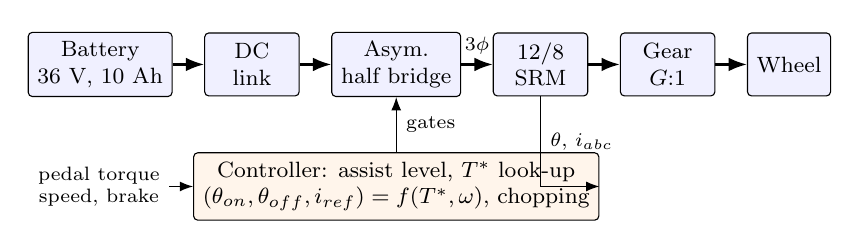
\begin{tikzpicture}[
  font=\footnotesize, >=Latex,
  blk/.style={draw, rounded corners=1.5pt, minimum height=8mm, minimum width=12mm, align=center, fill=blue!6},
  ctl/.style={draw, rounded corners=1.5pt, minimum height=7mm, align=center, fill=orange!8}]
\node[blk] (bat) {Battery\\36~V, 10~Ah};
\node[blk, right=4mm of bat] (cap) {DC\\link};
\node[blk, right=4mm of cap, minimum width=15mm] (conv) {Asym.\\half bridge};
\node[blk, right=4mm of conv] (srm) {12/8\\SRM};
\node[blk, right=4mm of srm] (gear) {Gear\\$G{:}1$};
\node[blk, right=4mm of gear, minimum width=9mm] (wheel) {Wheel};
\draw[->, thick] (bat) -- (cap);
\draw[->, thick] (cap) -- (conv);
\draw[->, thick] (conv) -- node[above]{\scriptsize 3$\phi$} (srm);
\draw[->, thick] (srm) -- (gear);
\draw[->, thick] (gear) -- (wheel);
\node[ctl, below=7mm of conv, minimum width=40mm] (ctrl) {Controller: assist level, $T^*$ look-up\\$(\theta_{on},\theta_{off},i_{ref})=f(T^*,\omega)$, chopping};
\draw[->] (ctrl.north) -- node[right]{\scriptsize gates} (conv.south);
\draw[->] (srm.south) |- node[pos=0.25, right]{\scriptsize $\theta$, $i_{abc}$} (ctrl.east);
\node[left=3mm of ctrl, align=center, font=\scriptsize] (ped) {pedal torque\\speed, brake};
\draw[->] (ped) -- (ctrl);
\end{tikzpicture}}
\caption{Architecture of the SRM-based pedelec drive.}
\label{fig:system}
\end{figure}

\subsection{Road-Load Model}
The tractive force at the tire contact patch is
\begin{equation}
F = C_{rr} m g\cos\alpha + m g \sin\alpha + \tfrac12 \rho C_dA\, v^2 + k_m m\, \dot v,
\label{eq:roadload}
\end{equation}
where $m=100$~kg (80-kg rider plus 20-kg bicycle), $C_{rr}=0.006$,
$C_dA=0.5$~m$^2$ (upright rider), $k_m=1.05$ accounts for rotating inertia,
and $\alpha=\arctan(\text{grade})$. With wheel radius $r_w=0.33$~m and gear
efficiency $\eta_g=0.95$, the motor torque and speed are
\begin{equation}
T_m = \frac{F r_w}{G\,\eta_g}, \qquad \omega_m = \frac{G v}{r_w}.
\label{eq:motortorque}
\end{equation}

\subsection{Duty Points}
Table~\ref{tab:duty} lists the motor-side requirements for $G=8$. Cruising on
level ground at 25~km/h needs only 149~W. Launching on an 8\% grade at
0.5~m/s$^2$ without rider effort, the worst case for throttle or walk-assist use,
needs 5.93~N$\cdot$m. This is four times the rated torque.

\begin{table}[!t]
\caption{Motor-Side Drive Requirements ($G = 8$)}
\label{tab:duty}
\centering
\renewcommand{\arraystretch}{1.1}
\begin{tabular}{l l r}
\hline
Duty point & Condition & Torque (N$\cdot$m)\\
\hline
Cruise & level, 25 km/h (149 W) & 0.88\\
Rated & 250 W at 25 km/h & 1.48\\
Hill & 6\% grade, 15 km/h & 3.03\\
Launch & 8\% grade, 0.5 m/s$^2$ & 5.93\\
\hline
Base speed $n_b$ & 25 km/h & 1608 r/min\\
Corner speed $n_c$ & $P_{pk}/T_{pk}$, $P_{pk}=500$ W & 805 r/min\\
Max.\ speed & 1.2 $n_b$ & 1930 r/min\\
\hline
\end{tabular}
\end{table}

\subsection{Corner-Speed Design Rule}
\label{sec:corner}
In single-pulse operation, the peak flux linkage a phase can reach is limited by
the volt-seconds applied during the dwell angle $\theta_d$:
\begin{equation}
\psi_{pk} = \frac{V_{dc}\,\theta_d}{\omega}.
\label{eq:voltsec}
\end{equation}
The number of turns per phase follows from $\psi_{pk}=T_{ph}B_{sp}A_{p}$, where
$A_p$ is the stator-pole face area and $B_{sp}$ the design pole flux density.
The average torque is $T=(mN_r/2\pi)W_c$, where $W_c$ is the energy converted
per stroke, i.e., the area of the $\psi$--$i$ loop. With a loop-utilization
factor $k_c=W_c/(\psi_{pk}I_{pk})$ and $\theta_d$ equal to the stroke angle
$\varepsilon=2\pi/(mN_r)$, the power at the speed $\omega_c$ where the turns are
chosen is
\begin{equation}
P_c = T_{pk}\,\omega_c = \frac{mN_r}{2\pi}\,k_c\,\psi_{pk} I_{pk}\,\omega_c = k_c\,V_{dc}\,I_{pk}.
\label{eq:invariant}
\end{equation}
Equation \eqref{eq:invariant} has two consequences. First, the peak current
needed for a given corner power is fixed by the battery voltage, \emph{not by
machine size}. A larger machine has fewer turns at the same volt-seconds and
therefore saturates at a similar ampere-turn-to-current ratio. Second, choosing
the turns for full torque at the 25-km/h base speed would require
$P_c=T_{pk}\omega_b\approx1$~kW and twice the phase current. The launch torque is
only needed at walking speed, so the turns are chosen at the corner speed
$n_c=P_{pk}/T_{pk}=805$~r/min (12.5~km/h) with $P_{pk}=500$~W. Above $n_c$ the
drive operates at approximately constant power. The simulations of
Section~\ref{sec:trade} give $k_c=0.54$--$0.66$ across all nine design variants.

\section{Topology Selection and Machine Design}

\subsection{Pole Configuration}
Table~\ref{tab:poles} compares candidate configurations at the maximum speed. The
12/8 machine has the same number of strokes per revolution as the four-phase
8/6 but needs only six switches. Its two pole pairs per phase balance the radial
forces and shorten the flux paths, which suits the short, large-diameter hub
envelope. Its phase frequency (257~Hz) keeps iron losses moderate with 0.35-mm
laminations, whereas 16/12 and 24/16 machines~\cite{bilgin2012,jiang2017} double
this frequency at no benefit for a 250-W machine. The 6/4 machine has a
30$^\circ$ stroke, which causes large torque dips and makes starting on a grade
more difficult.

\begin{table}[!t]
\caption{Comparison of Pole Configurations at 1930 r/min}
\label{tab:poles}
\centering
\renewcommand{\arraystretch}{1.1}
\begin{tabular}{c c c c c c}
\hline
$N_s/N_r$ & $m$ & Stroke & Strokes/rev & $f_{ph}$ (Hz) & Switches\\
\hline
6/4 & 3 & 30$^\circ$ & 12 & 129 & 6\\
8/6 & 4 & 15$^\circ$ & 24 & 193 & 8\\
\textbf{12/8} & \textbf{3} & \textbf{15$^\circ$} & \textbf{24} & \textbf{257} & \textbf{6}\\
16/12 & 4 & 7.5$^\circ$ & 48 & 386 & 8\\
24/16 & 3 & 7.5$^\circ$ & 48 & 514 & 6\\
\hline
\end{tabular}
\end{table}

\subsection{Main Dimensions}
In torque form, the SRM output equation~\cite{krishnan2001,krishnan1988} reads
\begin{equation}
T = \frac{\pi}{4}\,k_e\,k_d\,k_2\,B\,A\,D^2L,
\label{eq:output}
\end{equation}
where $D$ is the bore diameter and $L$ the stack length. The coefficients are
$k_e=0.85$ (efficiency), $k_d=0.9$ (duty), $k_2=0.7$ ($=1-1/\lambda_u$), $B=1.7$~T
(stator-pole flux density at alignment) and $A=45$~kA/m (short-term peak electric
loading). For $T_{pk}=5.93$~N$\cdot$m this gives $D^2L=184$~cm$^3$. An aspect
ratio $L/D=0.5$ and a split ratio $D/D_o=0.53$ give $D=71.7$~mm,
$L=35.9$~mm and $D_o=135.3$~mm. We use \eqref{eq:output} only as a starting
point. Its coefficients are optimistic for small, heavily saturated machines,
so the current required to meet $T_{pk}$ is determined by simulation
(Section~\ref{sec:flow}).

\subsection{Pole Arcs}
The stator and rotor pole arcs must satisfy the feasibility conditions of
Lawrenson \emph{et al.}~\cite{lawrenson1980}:
\begin{equation}
\min(\beta_s,\beta_r)\ge \varepsilon, \quad \beta_s\le\beta_r, \quad \beta_s+\beta_r<\frac{2\pi}{N_r}.
\label{eq:lawrenson}
\end{equation}
The first condition guarantees self-starting from every rotor position. The
second preserves slot area. The third creates a zero-overlap region that keeps
the unaligned inductance low. We select $\beta_s=15^\circ$ and $\beta_r=17^\circ$,
close to the lower-left vertex of the feasible region in Fig.~\ref{fig:geometry}(b).
This choice maximizes the inductance ratio and slot area. The $2^\circ$
excess of $\beta_r$ creates a short dwell before alignment in which the
tail current can decay before negative torque is produced.

\begin{figure}[!t]
\centering
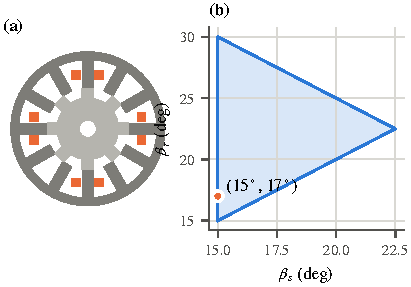
\includegraphics[width=\columnwidth]{fig_geometry}
\caption{(a) Lamination of the designed 12/8 SRM with phase-A coil sides marked.
(b) Feasible pole-arc region \eqref{eq:lawrenson} and the selected point.}
\label{fig:geometry}
\end{figure}

\subsection{Poles, Yokes, Turns and Winding}
The stator yoke is $y_s=0.75\,w_s$, where $w_s=9.4$~mm is the stator-pole width.
The pole flux divides in two in the yoke, so $0.5\,w_s$ is the minimum. The extra
margin limits yoke saturation and stiffens the stator against the ovalizing
vibration mode, which is the dominant source of SRM noise~\cite{miller1993}.
The rotor-pole height is limited to $30g$ ($g=0.3$~mm) as a compromise between
unaligned inductance and pole stiffness.

With \eqref{eq:voltsec} at $n_c$, the minimum battery voltage of 30~V and a
one-stroke dwell, $\psi_{pk}=93.2$~mWb. This gives $T_{ph}=164$ turns, i.e., 41
turns on each of the four poles of a phase. Bobbin-wound concentrated coils
with a net fill factor of 0.45 use 1.66-mm wire. The mean turn length is
115~mm and $R_{ph}=0.198~\Omega$ at 100~$^\circ$C. Table~\ref{tab:design}
summarizes the design.

\begin{table}[!t]
\caption{Main Parameters of the Designed 12/8 SRM}
\label{tab:design}
\centering
\renewcommand{\arraystretch}{1.08}
\setlength{\tabcolsep}{4pt}
\begin{tabular}{l r | l r}
\hline
Outer diameter & 135.3 mm & Turns/pole & 41\\
Bore diameter & 71.7 mm & Wire diameter & 1.66 mm\\
Stack length & 35.9 mm & $R_{ph}$ (100 $^\circ$C) & 0.198 $\Omega$\\
Air gap & 0.30 mm & $L_a$ (unsat.) & 9.06 mH\\
$\beta_s$ / $\beta_r$ & 15$^\circ$ / 17$^\circ$ & $L_u$ & 1.37 mH\\
Stator pole width & 9.36 mm & $L_a/L_u$ & 6.6\\
Stator pole height & 24.8 mm & $\psi_k$ & 85.3 mWb\\
Rotor pole height & 9.0 mm & Iron mass & 2.31 kg\\
Stator/rotor yoke & 7.0/19.1 mm & Copper mass & 1.09 kg\\
Slot area & 394 mm$^2$ & Rotor inertia & 4.1$\times$10$^{-4}$ kg$\cdot$m$^2$\\
\hline
\end{tabular}
\end{table}

\subsection{Inductances}
The aligned unsaturated inductance follows from two air gaps in series per pole
pair, with all $p=N_s/m$ poles of a phase in series:
\begin{equation}
L_a = k_{fe}\,\frac{\mu_0 (w_s+2g) L\, T_{ph}^2}{p\,g},
\label{eq:La}
\end{equation}
where $k_{fe}=0.9$ accounts for iron MMF and the $2g$ term for fringing. In
the unaligned position, the flux crosses into the rotor slot (path length $g+h_r$)
in parallel with two side paths to the neighboring rotor-pole corners
(path length $l_s$). This gives
\begin{equation}
\frac{L_u}{L_a} = \frac{k_{ew}}{k_{fe}}\left(\frac{g}{g+h_r}+\frac{g}{l_s}\right),
\label{eq:Lu}
\end{equation}
where $k_{ew}=1.35$ covers end-winding and slot leakage. The result,
$L_a/L_u=6.6$, is typical of small 12/8 machines with this air gap.

\section{Drive Modeling}

\subsection{Saturable Flux-Linkage Model}
The aligned magnetization curve is represented by an exponential knee
model in the spirit of~\cite{torrey1990,ilic1987}:
\begin{equation}
\psi_a(i) = L_{sat}\,i + \psi_k\left(1-e^{-(L_a-L_{sat})i/\psi_k}\right),
\label{eq:psia}
\end{equation}
whose slope is $L_a$ at $i=0$ and $L_{sat}$ in deep saturation. The knee flux is
$\psi_k=B_kA_pT_{ph}$ with $B_k=1.55$~T. A position function
$w(\theta)\in[0,1]$ blends \eqref{eq:psia} with the linear unaligned
characteristic:
\begin{equation}
\psi(i,\theta)=L_u i + w(\theta)\left[\psi_a(i)-L_u i\right].
\label{eq:psi}
\end{equation}
Here $w$ is unity while the stator pole is fully covered and zero without
overlap. Between these, it follows a $C^1$ smooth step that is widened by a
fringing angle of $2g/r$. Because $w$ multiplies a function of $i$ alone, the
co-energy and torque have closed forms:
\begin{align}
W'(i,\theta)&=\tfrac12 L_u i^2 + w(\theta)\big[W'_a(i)-\tfrac12 L_u i^2\big],\\
T(i,\theta)&=\frac{dw}{d\theta}\Big[W'_a(i)-\tfrac12 L_u i^2\Big],
\label{eq:torque}
\end{align}
with $W'_a(i)=\int_0^i\psi_a\,di$. Fig.~\ref{fig:static} shows the
magnetization curves and the static torque. Torque is concentrated in the
overlap region and grows sub-quadratically with current once the poles saturate.

\begin{figure}[!t]
\centering
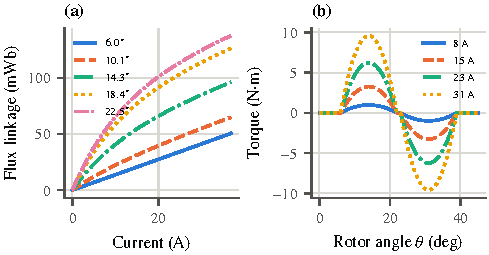
\includegraphics[width=\columnwidth]{fig_static}
\caption{(a) Flux linkage versus current from the onset of pole overlap (6.0$^\circ$) to
the aligned (22.5$^\circ$) position. (b) Static torque of one phase.}
\label{fig:static}
\end{figure}

\subsection{Converter and Circuit Model}
Each phase obeys $d\psi/dt = v-R_{ph}i$, with the converter imposing
\begin{equation}
v=\begin{cases}
\;\;V_{dc}-2R_{ds}i & \text{both switches on (magnetize)}\\
-(R_{ds}i+V_D) & \text{one switch on (freewheel)}\\
-(V_{dc}+2V_D) & \text{both off, }i>0\text{ (demagnetize)}
\end{cases}
\label{eq:states}
\end{equation}
with $R_{ds}=4$~m$\Omega$ and $V_D=0.8$~V. The flux equation is integrated at
40~kHz or at least 1800 steps per period, with $i$ obtained from
\eqref{eq:psi} by Newton iteration. A sampled hysteresis controller with a 2\%
band regulates the current by soft chopping. At high speed the back-EMF prevents
the reference from being reached, and single-pulse operation follows naturally.
Phases are identical and displaced by $\varepsilon$, so one phase is simulated
to periodic steady state and the total torque is
\begin{equation}
T_e(\theta)=\sum_{k=0}^{m-1}T_{ph}(\theta-k\varepsilon).
\label{eq:sum}
\end{equation}
The DC-link current is reconstructed in the same way. As a verification, the
DC input power equals the sum of electromagnetic power, copper loss and
conduction loss to within 1.1\% at all speeds from 80 to 1900~r/min.

\subsection{Loss Models}
Copper loss is $mR_{ph}I_{rms}^2$. Converter conduction loss is integrated from
\eqref{eq:states}, and switching loss is $\tfrac12V_{dc}I\,t_{sw}f_{sw}$ per
transition with $t_{sw}=60$~ns. Iron loss in the stator poles, stator yoke and
rotor is computed with the Bertotti form~\cite{bertotti1988}
\begin{equation}
p_{fe}=k_{ns}\left(k_h f B^2 + k_e (fB)^2\right)\quad\text{(W/kg)},
\label{eq:iron}
\end{equation}
calibrated to 2.7~W/kg at 1.5~T/50~Hz (M270-35A). Here $k_{ns}=1.3$ accounts
for the unipolar, non-sinusoidal SRM flux, $f=N_rn/60$ in the stator and
$N_sn/120$ in the rotor. Bearing and windage losses are below 2~W.

\section{Control and Design Flow}
\label{sec:flow}

\subsection{Commutation-Angle Optimization}
The turn-on angle must lead the start of pole overlap $\theta_{ov}$ by roughly
the angle needed to build up the reference current in $L_u$:
\begin{equation}
\theta_{adv}\approx \frac{\omega L_u i_{ref}}{V_{dc}-(R_{ph}+2R_{ds})i_{ref}}.
\label{eq:adv}
\end{equation}
At each speed--torque point $(\omega,T^*)$, we solve
\begin{equation}
\begin{aligned}
&\min_{\theta_{on},\theta_{off},i_{ref}} P_{in}\\
&\text{s.t.}\;\; \bar T_e=T^*,\;\; i_{ref}\le I_{max},\;\; \theta_{off}-\theta_{on}\le 0.55\,\tau_r,
\end{aligned}
\label{eq:opt}
\end{equation}
where $\tau_r=2\pi/N_r$. The search covers
$\theta_{on}\in[\theta_{ov}-1.6\,\theta_{adv},\,\theta_{ov}]$ and $\theta_{off}$
at 45--95\% of the interval from overlap to alignment. For each angle pair,
$i_{ref}$ is found with Brent's method. The dwell constraint is essential.
Without it, the optimizer drifts into continuous conduction at high speed, and the
tail current then produces negative torque after alignment. In a controller,
the solution becomes a two-dimensional look-up table
$(\theta_{on},\theta_{off},i_{ref})=f(T^*,\omega)$, as in~\cite{kjaer1997,xue2010}.

\subsection{Design Flow}
Fig.~\ref{fig:flow} summarizes the procedure. The analytical machine design is
followed by a simulation step that finds the smallest current giving
$T_{pk}$ with optimal angles. Here this current is 27.9~A. The converter
limit is set 10\% higher, at $I_{max}=30.7$~A.

\begin{figure}[!t]
\centering
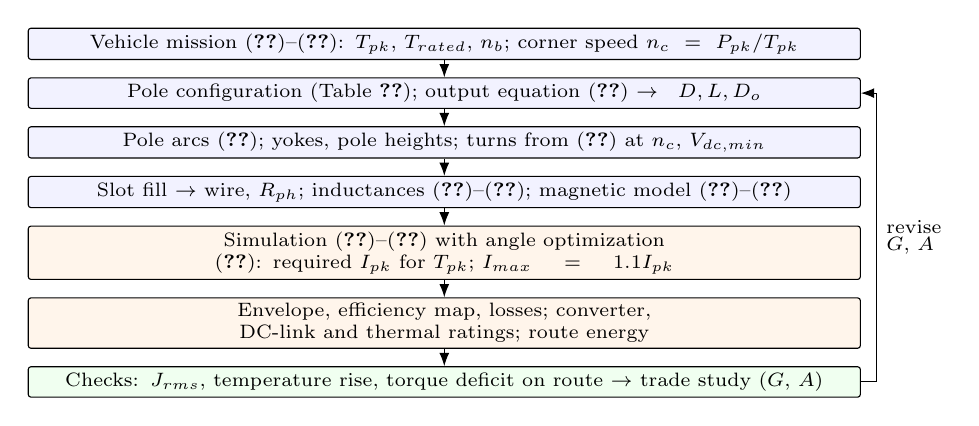
\begin{tikzpicture}[font=\scriptsize, >=Latex, node distance=2.2mm,
  st/.style={draw, rounded corners=1pt, align=center, text width=0.86\columnwidth, fill=blue!5, inner sep=2pt}]
\node[st] (a) {Vehicle mission \eqref{eq:roadload}--\eqref{eq:motortorque}: $T_{pk}$, $T_{rated}$, $n_b$; corner speed $n_c=P_{pk}/T_{pk}$};
\node[st, below=of a] (b) {Pole configuration (Table~\ref{tab:poles}); output equation \eqref{eq:output} $\rightarrow D, L, D_o$};
\node[st, below=of b] (c) {Pole arcs \eqref{eq:lawrenson}; yokes, pole heights; turns from \eqref{eq:voltsec} at $n_c$, $V_{dc,min}$};
\node[st, below=of c] (d) {Slot fill $\rightarrow$ wire, $R_{ph}$; inductances \eqref{eq:La}--\eqref{eq:Lu}; magnetic model \eqref{eq:psia}--\eqref{eq:psi}};
\node[st, below=of d, fill=orange!8] (e) {Simulation \eqref{eq:states}--\eqref{eq:sum} with angle optimization \eqref{eq:opt}: required $I_{pk}$ for $T_{pk}$; $I_{max}=1.1I_{pk}$};
\node[st, below=of e, fill=orange!8] (f) {Envelope, efficiency map, losses; converter, DC-link and thermal ratings; route energy};
\node[st, below=of f, fill=green!6] (g) {Checks: $J_{rms}$, temperature rise, torque deficit on route $\rightarrow$ trade study ($G$, $A$)};
\foreach \u/\v in {a/b,b/c,c/d,d/e,e/f,f/g} \draw[->] (\u) -- (\v);
\draw[->] (g.east) -- ++(2mm,0) |- node[pos=0.25, right, align=left]{\scriptsize revise\\[-2pt]\scriptsize $G$, $A$} (b.east);
\end{tikzpicture}
\caption{Mission-to-converter design flow of the SRM e-bike drive.}
\label{fig:flow}
\end{figure}

\section{Results}

\subsection{Current and Torque Waveforms}
Fig.~\ref{fig:waveforms} shows the steady-state waveforms in the two operating
modes. At launch (80~r/min), soft chopping holds the current at 30.7~A. The pole
saturates ($B_{sp}\approx2$~T), and late commutation ($\theta_{off}=21.7^\circ$)
uses most of the stroke, giving a mean torque of 6.81~N$\cdot$m. At the rated point
(1608~r/min), the turn-on angle is advanced to $-4.9^\circ$. The current peaks
early, and the flux rises linearly to 57~mWb at turn-off. The peak-to-peak torque
ripple is 113\% at launch and 148\% at the rated point. This is inherent to a
three-phase machine with $\beta_s=\varepsilon$ under current-reference control, and
it is discussed in Section~\ref{sec:discussion}.

\begin{figure*}[!t]
\centering
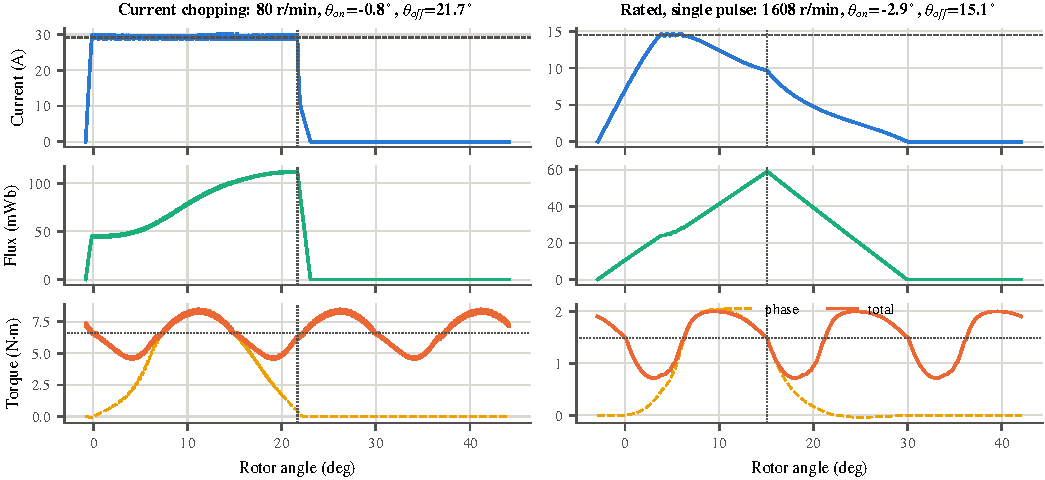
\includegraphics[width=\textwidth]{fig_waveforms}
\caption{Steady-state phase current, flux linkage and torque (single phase and
total) at launch (left, current chopping) and at the rated point (right,
single pulse). Dotted vertical lines mark $\theta_{off}$.}
\label{fig:waveforms}
\end{figure*}

\subsection{Torque--Speed Capability}
At $I_{max}=30.7$~A, the envelope in Fig.~\ref{fig:ts} delivers 6.8~N$\cdot$m at
low speed and about 3.6~N$\cdot$m at 25~km/h. The available power exceeds the
500-W target above about 900~r/min. All duty points of Table~\ref{tab:duty} lie
inside the envelope. A steady 8\% climb at more than about 20~km/h without
rider input lies outside it. This is consistent with the pedelec concept, in which
the rider contributes on steep grades.

\begin{figure}[!t]
\centering
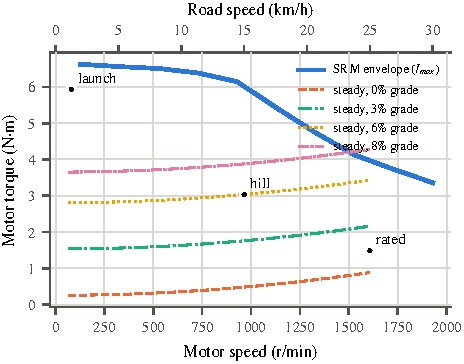
\includegraphics[width=\columnwidth]{fig_torque_speed}
\caption{Torque envelope at $I_{max}$ with optimized angles, steady road-load
torque for 0--8\% grades, and the duty points of Table~\ref{tab:duty}.}
\label{fig:ts}
\end{figure}

\subsection{Efficiency and Losses}
Fig.~\ref{fig:map} shows the battery-to-shaft efficiency map with the operating
points of the route of Section~\ref{sec:route} overlaid. The maximum system
efficiency is 78.6\% and the maximum motor efficiency 81.4\%. Both occur at
medium torque near and above the base speed, which is where the route's cruise
and rated points lie. Table~\ref{tab:ops} and Fig.~\ref{fig:losses} give the operating
points and their loss breakdown. Copper loss dominates everywhere. This is the
characteristic SRM penalty: the stator also carries the magnetizing current,
as unipolar pulses with a high RMS-to-average ratio. At the rated point, iron
loss accounts for about 21\% and converter conduction loss for about 14\% of the
86-W total. The diode drops are significant at only 36~V.

\begin{figure}[!t]
\centering
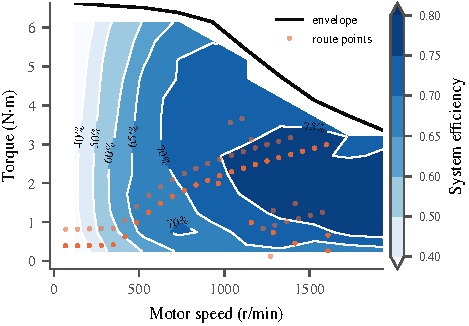
\includegraphics[width=\columnwidth]{fig_efficiency_map}
\caption{Battery-to-shaft efficiency map (optimized angles at each point), with
the torque envelope and the operating points of the route simulation.}
\label{fig:map}
\end{figure}

\begin{table}[!t]
\caption{Optimized Operating Points}
\label{tab:ops}
\centering
\renewcommand{\arraystretch}{1.1}
\setlength{\tabcolsep}{3.5pt}
\begin{tabular}{l r r r r r r r}
\hline
Point & $n$ & $\bar T_e$ & $\theta_{on}$ & $\theta_{off}$ & $I_{rms}$ & $\eta_{mot}$ & $\eta_{sys}$\\
 & r/min & N$\cdot$m & deg & deg & A & \% & \%\\
\hline
Launch & 80 & 6.81 & 4.5 & 21.7 & 18.9 & 20.7 & 18.8\\
Hill 6\% & 965 & 3.03 & $-0.5$ & 17.6 & 12.1 & 73.4 & 70.8\\
Rated & 1608 & 1.48 & $-4.9$ & 17.6 & 9.5 & 75.8 & 72.8\\
Cruise & 1608 & 0.88 & $-4.9$ & 17.6 & 6.8 & 75.6 & 71.6\\
\hline
\end{tabular}
\end{table}

\begin{figure}[!t]
\centering
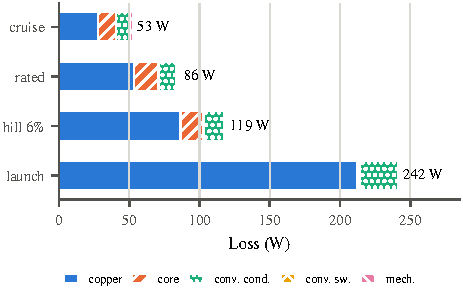
\includegraphics[width=\columnwidth]{fig_losses}
\caption{Loss breakdown at the operating points of Table~\ref{tab:ops}.}
\label{fig:losses}
\end{figure}

\subsection{Converter Design}
The asymmetric half bridge (two switches and two diodes per phase) is the only
common SRM converter that provides $+V_{dc}$, $0$ and $-V_{dc}$ independently in
every phase. These states allow fast demagnetization, soft chopping and
phase-independent fault handling~\cite{krishnan2001,miller1993}. The
$(n{+}1)$-switch and Miller converters share a switch, which prevents phase
overlap at speed and forces hard chopping. The C-dump converter needs an extra
inductor and capacitor, and the split-DC converter halves the phase voltage
and needs an even number of phases. Table~\ref{tab:conv} lists the ratings.
The DC-link capacitor is dimensioned by ripple current rather than by
capacitance. The SRM draws unipolar pulses, and during demagnetization the
energy returns to the link. The resulting ripple current exceeds the
average battery current. The average hysteresis switching frequency is
2.4--6~kHz, which is audible. A production design should use fixed-frequency
($\ge$16~kHz) PWM current control with the same soft-chopping states.

\begin{table}[!t]
\caption{Converter and DC-Link Ratings}
\label{tab:conv}
\centering
\renewcommand{\arraystretch}{1.1}
\begin{tabular}{l r}
\hline
Device voltage ($1.5\,V_{bat,max}$) / selected & 63 V / 100 V MOSFET\\
Phase current limit $I_{max}$ & 30.7 A\\
Device RMS current at launch & 18.9 A\\
Average battery current, rated / launch & 8.7 A / 8.2 A\\
DC-link ripple current (RMS), rated / launch & 10.9 A / 15.4 A\\
DC-link capacitance for $\le$5\% voltage ripple & 3.8 mF\\
\hline
\end{tabular}
\end{table}

\subsection{Thermal Assessment}
At the continuous rated point the motor dissipates 73~W. The current density is
4.4~A/mm$^2$. The hub shell provides 0.075~m$^2$ of cooling surface, and riding
gives a convection coefficient of about 25~W/m$^2$K. A lumped model then
predicts a temperature rise of 39~K, or a winding hot spot of about
77~$^\circ$C at 30~$^\circ$C ambient. This leaves a wide margin to class-F
insulation for sustained climbing. The launch point (240~W loss) is limited
to tens of seconds by the thermal capacity of the copper (about 420~J/K).
Because the rotor contains no magnets, the machine tolerates these transients
without risk of demagnetization.

\section{Route Energy Evaluation}
\label{sec:route}
A 6.4-km urban route with five stops, a 700-m climb at 6\% and a 900-m descent at
$-4$\% was simulated quasi-statically (Fig.~\ref{fig:cycle}). The rider supplies
up to 100~W, force-limited at low speed. The motor supplies the remaining
tractive power below 25~km/h, with efficiency interpolated from
Fig.~\ref{fig:map}, and braking is mechanical. The ride takes 18.9~min. The rider
contributes 25.5~Wh and the motor 23.4~Wh at the shaft, which draws 32.3~Wh from
the battery. The cycle-average drive efficiency is therefore 72.3\%. Consumption is
5.05~Wh/km, which corresponds to about 64~km of range from 90\% of a 360-Wh pack.
The torque demand never exceeded the envelope. Launches briefly reach about
3.7~N$\cdot$m and 660~W of battery power.

\begin{figure}[!t]
\centering
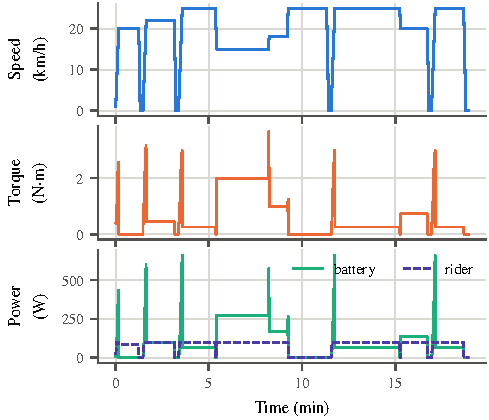
\includegraphics[width=\columnwidth]{fig_cycle}
\caption{Route simulation: speed, motor torque, and battery and rider power.}
\label{fig:cycle}
\end{figure}

\section{Design Trade-Offs}
\label{sec:trade}
Table~\ref{tab:trade} and Fig.~\ref{fig:trade} vary the gear ratio $G$ and the
peak electric loading $A$, redesigning the machine and repeating the current
sizing each time. Three observations stand out.
\begin{enumerate}
\item The required peak current varies only from 27.7 to 33.7~A across a
fourfold range of active mass, as predicted by \eqref{eq:invariant}.
\item Efficiency is governed mainly by electric loading. Each step from 60 to
45 to 35~kA/m adds about five points of rated efficiency for about 30\% more mass.
\item A higher gear ratio reduces machine size. The variant with $G=11$ and $A=35$~kA/m
has the baseline's diameter (132~mm) and slightly lower mass (3.2~kg), yet
gains about four points of system efficiency. The cost is a two-stage gear and a
higher iron-loss frequency.
\end{enumerate}
The single-stage $G=8$, $A=45$~kA/m baseline favors cost and simplicity. The
$G=11$, $A=35$~kA/m variant is preferable when range is the priority.

\begin{table}[!t]
\caption{Trade Study: Gear Ratio $G$ and Peak Electric Loading $A$}
\label{tab:trade}
\centering
\renewcommand{\arraystretch}{1.1}
\setlength{\tabcolsep}{4pt}
\begin{tabular}{c c c c c c c c}
\hline
$G$ & $A$ & $D_o$ & $L$ & Mass & $I_{max}$ & $\eta_{mot}$ & $\eta_{sys}$\\
 & kA/m & mm & mm & kg & A & \% & \%\\
\hline
5 & 60 & 143.8 & 38.1 & 4.10 & 27.7 & 70.6 & 68.5\\
5 & 45 & 158.3 & 41.9 & 5.51 & 29.2 & 76.3 & 73.6\\
5 & 35 & 172.1 & 45.6 & 7.14 & 31.2 & 81.0 & 78.0\\
8 & 60 & 122.9 & 32.6 & 2.53 & 29.3 & 70.6 & 68.1\\
\textbf{8} & \textbf{45} & \textbf{135.3} & \textbf{35.9} & \textbf{3.40} & \textbf{30.7} & \textbf{75.8} & \textbf{72.8}\\
8 & 35 & 147.1 & 39.0 & 4.40 & 32.0 & 79.9 & 76.6\\
11 & 60 & 110.6 & 29.3 & 1.82 & 30.3 & 69.9 & 67.3\\
11 & 45 & 121.7 & 32.2 & 2.45 & 31.6 & 74.8 & 71.6\\
11 & 35 & 132.3 & 35.1 & 3.17 & 33.7 & 80.2 & 77.0\\
\hline
\end{tabular}
\end{table}

\begin{figure}[!t]
\centering
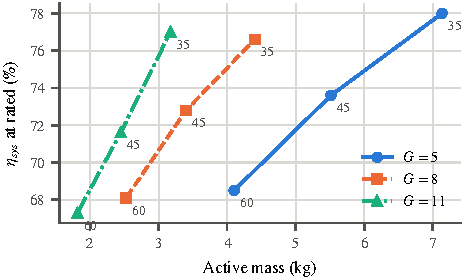
\includegraphics[width=\columnwidth]{fig_trade}
\caption{Rated-point system efficiency versus active mass for gear ratios 5, 8
and 11. The labels give the peak electric loading in kA/m.}
\label{fig:trade}
\end{figure}

\section{Discussion}
\label{sec:discussion}

\subsection{Torque Ripple and Acoustic Noise}
With $\beta_s=\varepsilon$ and flat-top current references, essentially one
phase conducts at a time, which explains the 110--150\% ripple. The gear and
wheel inertia filter much of it. On a bicycle frame, however, the residual is
felt as vibration and heard as noise, together with the radial-force excitation
of the stator. Mitigation options, in increasing order of cost, are as follows.
Torque-sharing functions overlap the incoming and outgoing phases and typically
reduce ripple to a few tens of percent at low speed for a modest increase in RMS
current~\cite{husain2002,vujicic2012,ye2015}. Wider rotor poles increase phase
overlap. Shaped or notched poles help further. On the mechanical side, a stiff,
round stator yoke and a compliant gear coupling reduce noise. The
look-up-table structure of Section~\ref{sec:flow} accommodates
torque-sharing references directly.

\subsection{Position Sensing}
Commutation needs rotor position to about 1$^\circ$ mechanical. Three Hall
sensors on a target ring provide 15$^\circ$ edges, which can be interpolated
using speed. Sensorless schemes based on flux observers or inductance
probing~\cite{ehsani2002} are attractive for sealed hubs. They must, however,
achieve reliable stand-still starts on a grade, which is exactly the launch
condition that sizes the drive.

\subsection{Mechanical Considerations}
The 0.3-mm air gap is small for a wheel hub that sees road shocks. It
requires a stiff axle, preloaded bearings on both sides of the stack and
careful tolerance analysis. Every additional 0.05~mm reduces $L_a$ by about
15\%. The magnet-free rotor ($4.1\times10^{-4}$~kg$\cdot$m$^2$) is robust at
overspeed and can be sealed without corrosion concerns. Because no drag torque
exists when unpowered, the freewheel clutch normally found in geared hubs becomes
optional.

\subsection{Comparison With PM Hub Drives and Limitations}
Commercial PM geared hubs of similar rating typically quote peak efficiencies in
the low-to-mid 80\% range. The SRM baseline trades several points of efficiency
for the absence of magnets and drag torque, lower material cost and fault
tolerance. The trade study shows that most of this gap can be closed by mass
or gearing. Further gains are possible from thinner (0.2-mm) laminations, a
0.25-mm air gap and segmented stators with fill factors above 0.5.

The results rest on analytical permeance estimates of $L_a$, $L_u$ and the knee
flux, on a lumped iron-loss model and on a one-node thermal model. We
estimate their uncertainty at about $\pm$15\% for inductance and torque and
$\pm$30\% for iron loss. Mutual coupling between phases is neglected, which is
justified for short-pitched concentrated coils. The flux-linkage model exposes
the same interface as a tabulated $\psi(i,\theta)$ characteristic, so
finite-element data can replace it directly. Finite-element verification and
prototype measurements are the next steps of this work.

\section{Conclusion}
This paper has presented the analysis and design of a switched reluctance
motor drive for a 250-W pedelec, from vehicle mission to converter. The key
design insight is the corner-speed rule. Choosing the turns at
$n_c=P_{pk}/T_{pk}$ rather than at the 25-km/h base speed halves the launch
current. The invariant $P_c=k_cV_{dc}I_{pk}$, with $k_c\approx0.54$--$0.66$, shows that
peak current is set by battery voltage and power rather than by machine size.
The resulting 12/8 SRM has an outer diameter of 135~mm and 3.4~kg of active
mass, and drives the wheel through an 8:1 gear from a three-phase asymmetric
half bridge with 100-V MOSFETs. It meets all duty points, including a
5.9-N$\cdot$m launch on an 8\% grade at 31~A. At the rated point it reaches 75.8\%
motor and 72.8\% system efficiency, and it consumes 5.05~Wh/km on a hilly urban
route, which corresponds to about 64~km of range. With higher gearing and lower electric
loading, efficiency rises to about 80\% at equal mass. These results indicate
that the SRM is a technically viable, magnet-free alternative for pedelec
drives, provided that torque ripple is handled by torque-sharing control and
careful mechanical design.

\bibliographystyle{IEEEtran}
\bibliography{references}

\end{document}
